\documentclass[/home/jesse/Analysis/FemtoAnalysis/AnalysisNotes/AnalysisNoteJBuxton.tex]{subfiles}

\renewcommand{\NonFlatBgdLamKch}{_NonFlatBgdCrctnLamK0LinearLamKchPolynomial}
\renewcommand{\NonFlatBgdLamKs}{_NonFlatBgdCrctnLamK0LinearLamKchPolynomial}

\renewcommand{\ResNum}{_NoRes}
\renewcommand{\PrimMaxDecay}{}
\renewcommand{\ResMethod}{}

\renewcommand{\SaveNameModLamKch}{\MomRes\NonFlatBgdLamKch\ResNum\PrimMaxDecay\ResMethod\ParamFixAndShareLamKch}
\renewcommand{\SaveNameModLamKs}{\MomRes\NonFlatBgdLamKs\ResNum\PrimMaxDecay\ResMethod\ParamFixAndShareLamKch}

\begin{document}

\subsection{No Residual Contributors Included in Fit}
\label{App_ResultsLamK_NoRes}

This section presents fit results for which no residual contributors were assumed.
This is a typical starting point for femtoscopic analyses such as ours, and the effects of residual contributions are sometimes ignored.
Therefore, it is interesting to observe the effects of neglecting residual feed-down from our fit description.
For a comparison of these results to the case of three residual contributors, see Fig. \ref{figApp:Comparisons_3v10vNo} in App. \ref{App_ResultsLamK_FitMethComp}

%%%%%%%%%%%%%%%%%%%%%%%%%%%%%%%%%%%%%%%%%%%%%%%%%%%%%%%%%%%%%%%%%%%%%%
\begin{figure}[h]
  \centering
  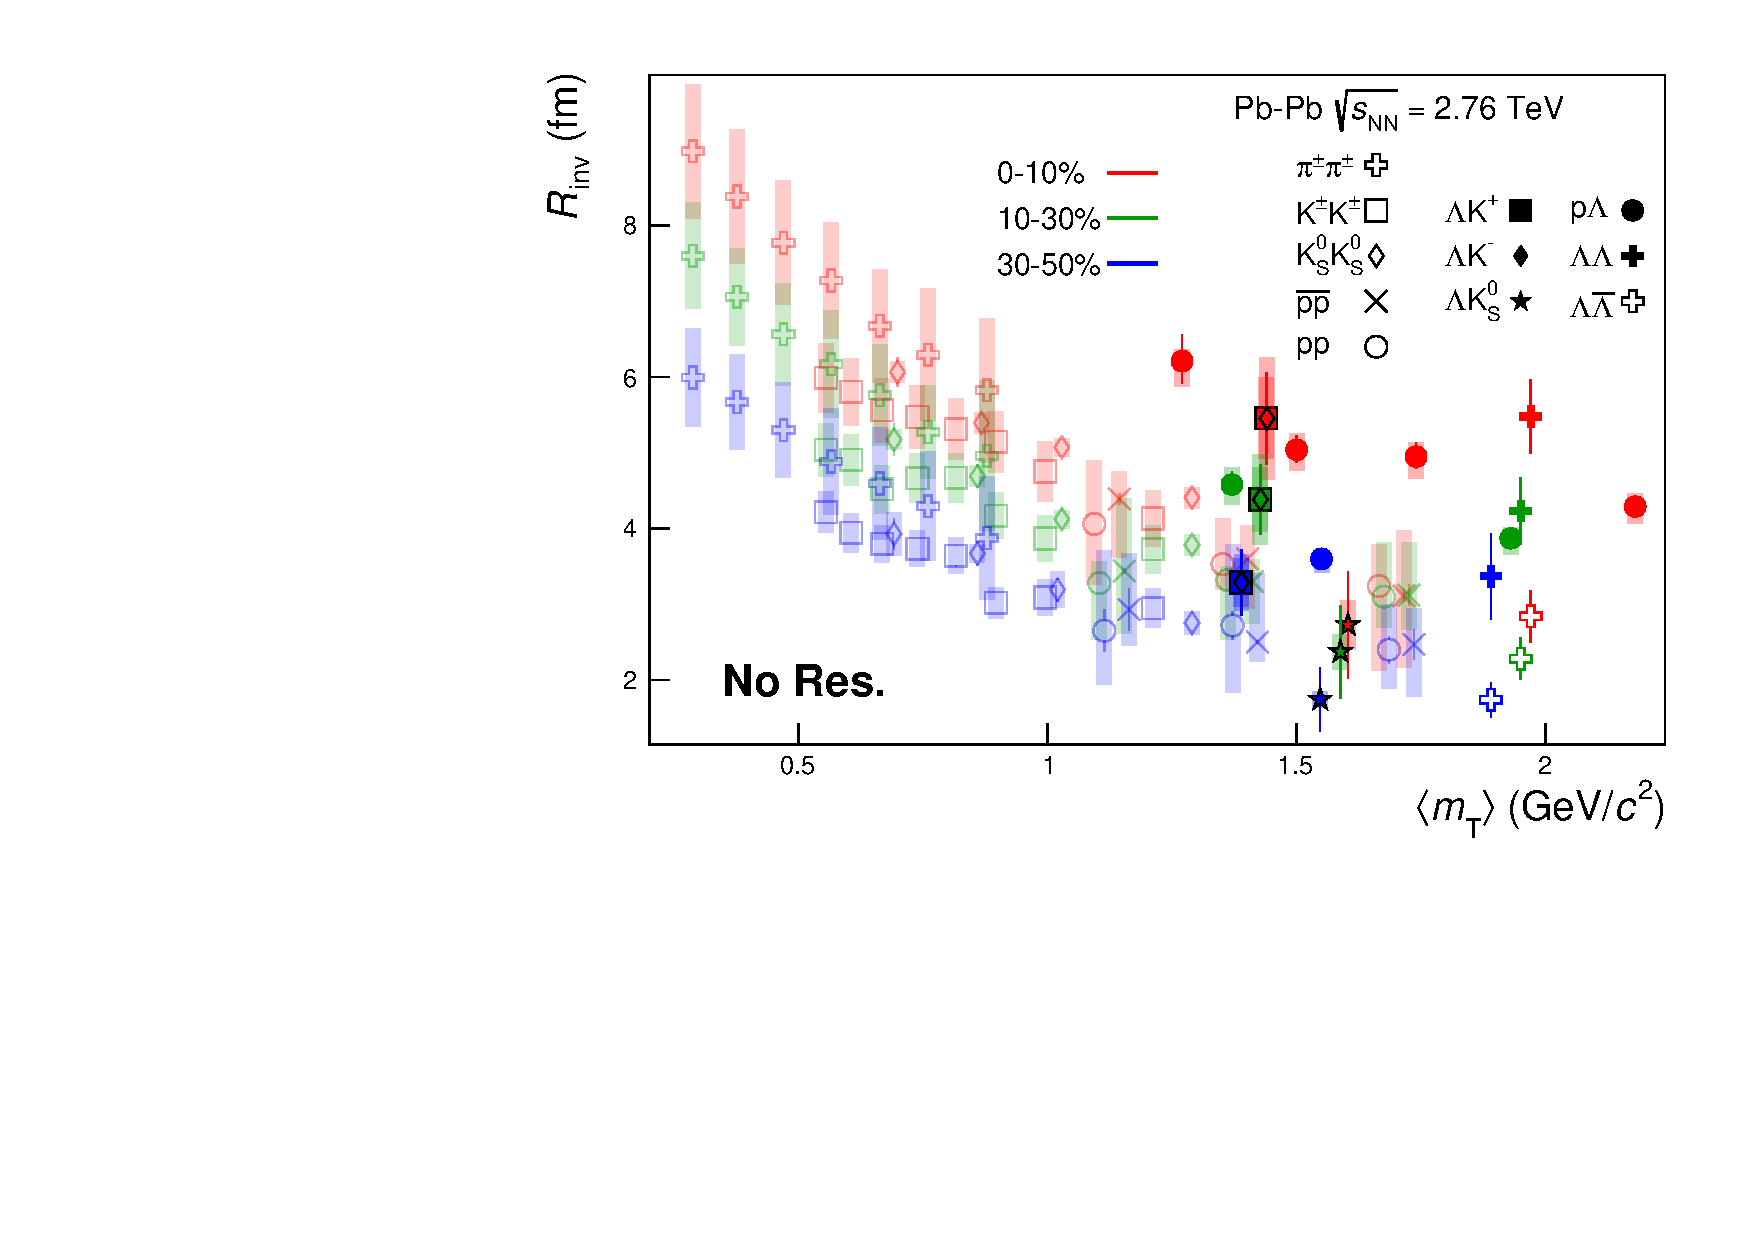
\includegraphics[width=0.80\textwidth]{\ResultsDirBaseLamKch\SaveNameModLamKch/Comparisons/mTscaling_MinvCalc_OutlinedPoints_OthersTransparent_wJaiAndHans_NoRes.pdf}
  \caption[$m_{\mathrm{T}}$ scaling of radii: No residuals]
  {
  No residual correlations in \LamK fits.  
  Extracted fit $R_{\mathrm{inv}}$ parameters as a function of pair transverse mass ($m_{\mathrm{T}}$) for various pair systems over several centralities. 
  The ALICE published data \cite{Adam:2015vja} are shown with transparent, open symbols.  
  The new \LamK results are shown with opaque, filled symbols.  
  The \mt value for the \LamK system is an average of those for the \LamKchP, \ALamKchM, and \LamKs systems.
  }
  \label{figApp:mTScalingOfRadii_NoRes}
\end{figure}

\begin{figure}[h]
  \centering
  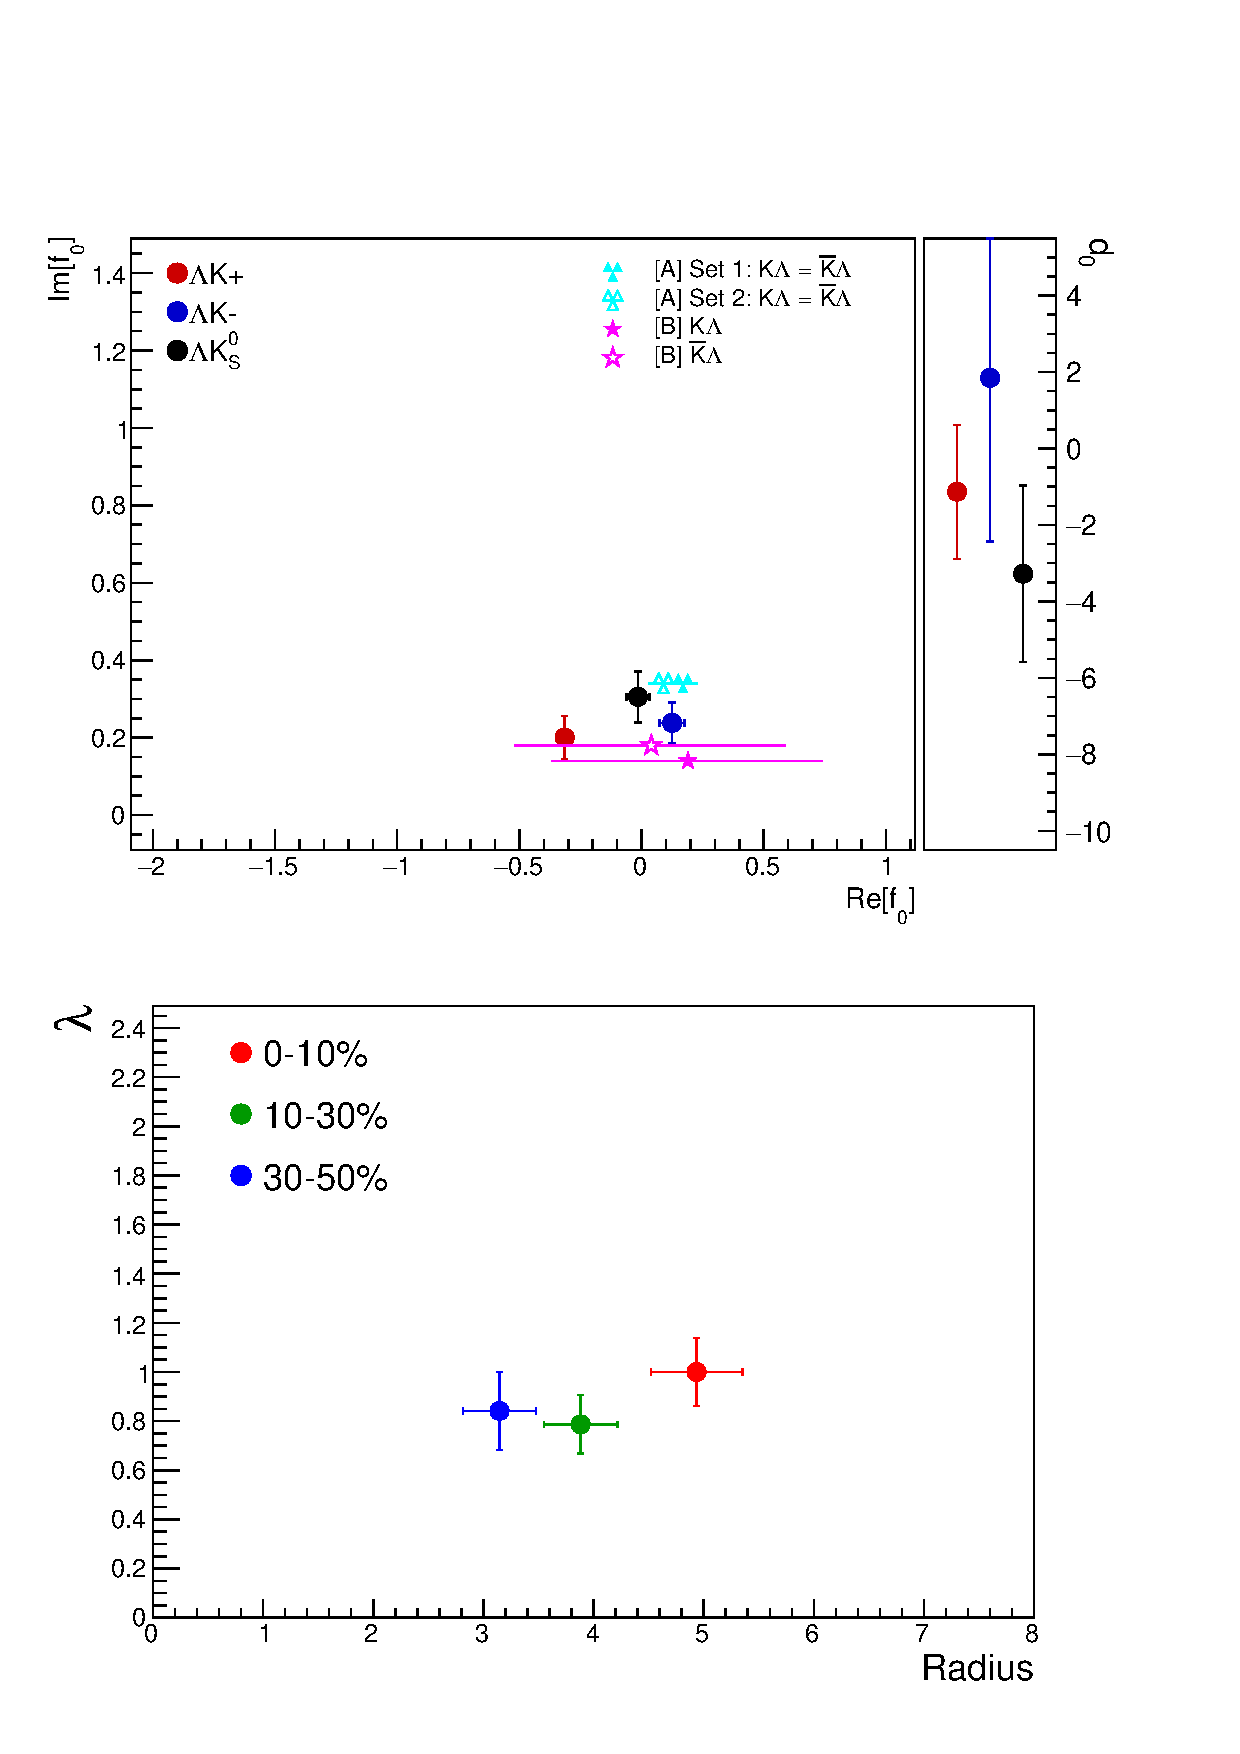
\includegraphics[width=0.65\textwidth]{\ResultsDirBaseLamKch\SaveNameModLamKch/Comparisons/FinalResults_Comp3An_StatOnly_Vertical.pdf}
  \caption[Extracted scattering parameters: No residuals]
  {
  Extracted fit parameters for the case of no residual contributors for all of our \LamK systems.  
  [Top]: $\Im f_{0}$ vs. $\Re f_{0}$, together with $d_{0}$ to the right.  
  [Bottom]: $\lambda$ vs. Radius for the 0-10\% (blue), 10-30\% (green), and 30-50\% (red) centrality bins.  
  In the fit, all \LamK systems share common radii.
  The color scheme used in the panel are to be consistent with those in Fig. \ref{figApp:mTScalingOfRadii_NoRes}.
  The cyan ([A] = Ref. \cite{Liu:2006xja}) and magenta ([B] = Ref. \cite{Mai:2009ce}) points show theoretical predictions made using chiral perturbation theory.
  }
  \label{figApp:ScattParams_NoRes}
\end{figure}

\begin{comment}
\begin{figure}[h]
  \centering
  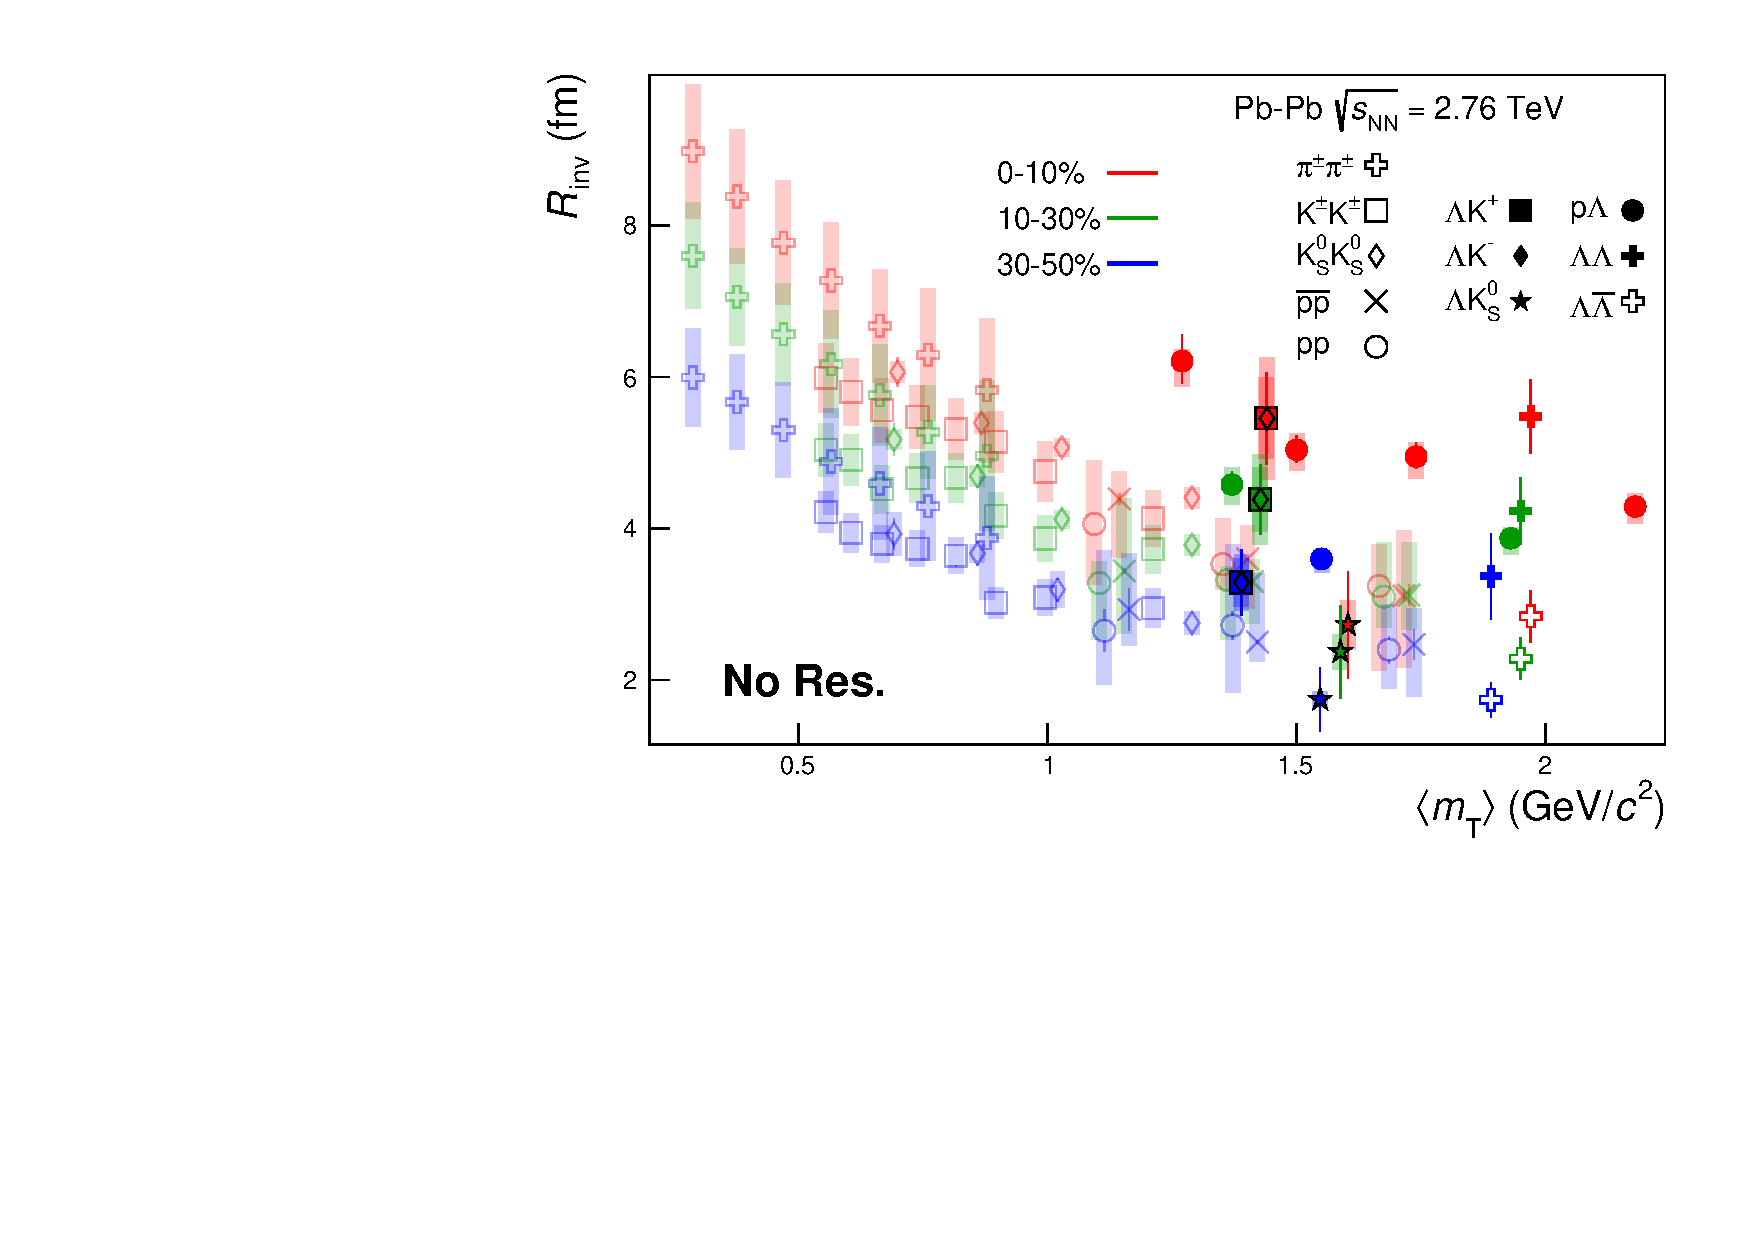
\includegraphics[width=0.80\textwidth]{\ResultsDirBaseLamKch\SaveNameModLamKch/Comparisons/mTscaling_MinvCalc_OutlinedPoints_OthersTransparent_wJaiAndHans_NoRes.pdf}
  \caption[$m_{\mathrm{T}}$ scaling of radii]
  {
  no residual correlations in \LamK fits.  
  Extracted fit $R_{\mathrm{inv}}$ parameters as a function of pair transverse mass ($m_{\mathrm{T}}$) for various pair systems over several centralities. 
  The ALICE published data \cite{Adam:2015vja} are shown with transparent, open symbols.  
  The new \LamK results are shown with opaque, filled symbols.  
  The \mt value for the \LamK system is an average of those for the \LamKchP, \ALamKchM, and \LamKs systems.
  }
  \label{figApp:mTScalingOfRadii_NoRes}
\end{figure}
\end{comment}

%%%%%%%%%%%%%%%%%%%%%%%%%%%%%%%%%%%%%%%%%%%%%%%%%%%%%%%%%%%%%%%%%%%%%%
\begin{figure}[h]
  \centering
  \includegraphics[width=0.75\textwidth]{\ResultsDirBaseLamKch\SaveNameModLamKch/canKStarCfwFitsLamKchPwConj_0010_1030_3050UnZoomed\SaveNameModLamKch.pdf}
  \caption[\LamKchPALamKchM data with fits: no residuals]
  {
  Fit results, with no residual correlations included, for the \LamKchP and \ALamKchM data.
  The \LamKchP data is shown in the left column, the \ALamKchM in the right, and the rows differentiate the different centrality bins (0-10\% in the top, 10-30\% in the middle, and 30-50\% in the bottom).
  }
  \label{figApp:LamKchPwConjFits_NoRes}
\end{figure}


%%%%%%%%%%%%%%%%%%%%%%%%%%%%%%%%%%%%%%%%%%%%%%%%%%%%%%%%%%%%%%%%%%%%%%
\begin{figure}[h]
  \centering
  \includegraphics[width=0.75\textwidth]{\ResultsDirBaseLamKch\SaveNameModLamKch/canKStarCfwFitsLamKchMwConj_0010_1030_3050UnZoomed\SaveNameModLamKch.pdf}
  \caption[\LamKchMALamKchP data with fits: no residuals]
  {
  Fit results, with no residual correlations included, for the \LamKchM and \ALamKchP data.
  The \LamKchM data is shown in the left column, the \ALamKchP in the right, and the rows differentiate the different centrality bins (0-10\% in the top, 10-30\% in the middle, and 30-50\% in the bottom).
  }
  \label{figApp:LamKchMwConjFits_NoRes}
\end{figure}


%%%%%%%%%%%%%%%%%%%%%%%%%%%%%%%%%%%%%%%%%%%%%%%%%%%%%%%%%%%%%%%%%%%%%%
\begin{figure}[h]
  \centering
  \includegraphics[width=0.75\textwidth]{\ResultsDirBaseLamKs\SaveNameModLamKs/canKStarCfwFitsLamK0wConj_0010_1030_3050UnZoomed\SaveNameModLamKs.pdf}
  \caption[\LamALamKs data with fits: no residuals]
  {
  Fit results, with no residual correlations included, for the \LamKs and \ALamKs data.
  The \LamKs data is shown in the left column, the \ALamKs in the right, and the rows differentiate the different centrality bins (0-10\% in the top, 10-30\% in the middle, and 30-50\% in the bottom).
  }
  \label{figApp:LamKswConjFits_NoRes}
\end{figure}


\begin{comment}
%%%%%%%%%%%%%%%%%%%%%%%%%%%%%%%%%%%%%%%%     TABLES!!!!!     %%%%%%%%%%%%%%%%%%%%%%%%%%%%%%%%%%%%%%%%
%\pagestyle{empty}
\begin{landscape}

\subfile{\ResultsDirBaseLamKs\SaveNameModLamKs/Tables/ResultsTable_cLamK0.tex}
\subfile{\ResultsDirBaseLamKch\SaveNameModLamKch/Tables/ResultsTable_cLamcKch.tex}

\end{landscape}
%\pagestyle{plain}
%%%%%%%%%%%%%%%%%%%%%%%%%%%%%%%%%%%%%%%%%%%%%%%%%%%%%%%%%%%%%%%%%%%%%%%%%%%%%%%%%%%%%%%%%%%%%%%%%%%%%
\end{comment}


\clearpage

\end{document}